This section will describe the overall structure of the Back Burner Brew. The Brew System Vessel layer is where the brewing process will take place and could function as its own brewing system without the automation. All the other layers are built on top of the Brew System Vessel layer and will be used to automate the brewing process.

\begin{figure}[H]
	\centering
	\graphicspath{.\images}
	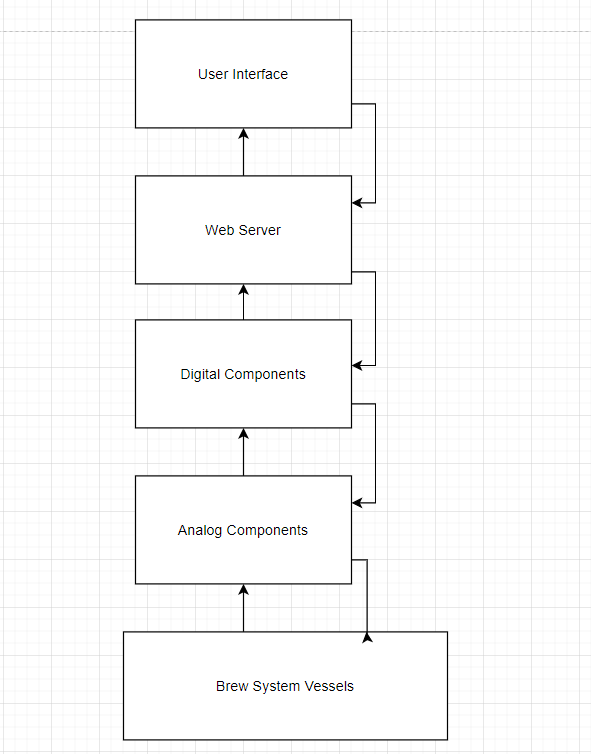
\includegraphics[scale=0.5]{images/simple_ads.PNG}
	\caption{Simple ADS}
\end{figure}
\subsection{Brew System Vessel Layer}

\begin{figure}[H]
	\centering
	\graphicspath{.\images}
	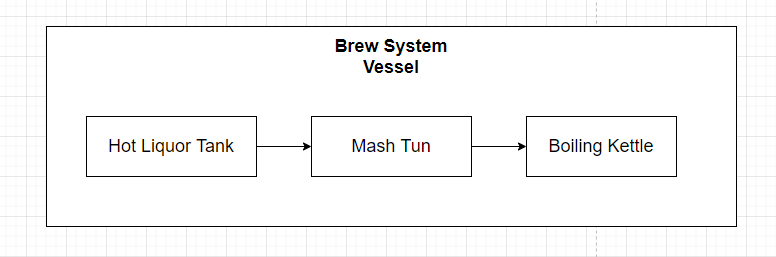
\includegraphics[scale=0.5]{images/brew_layer.PNG}
	\caption{Brew System Vessel Layer}
\end{figure}

The Brew System Vessel Layer is where the brewing process will take place and does not have any software involved. This layer would be enough for a brewer to make their own beer without any automation. This layer is comprised of the mash tun, hot liquor tank(HLT), and the brewing kettle. The HLT will control the temperature of the liquid inside the mash tun by heating the liquid through a coil inside the HLT. The mash tun is where the mashing process begins and the grain is added to the water. The boiling kettle is where the liquid will be boiled for a set amount of time and then sent to a chiller and fermentation kettle. 

\subsection{Analog Components Layer}
\begin{figure}[H]
	\centering
	\graphicspath{.\images}
	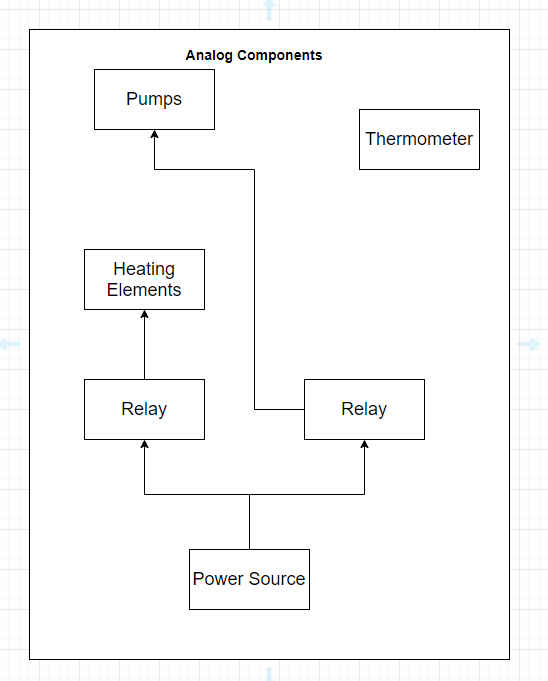
\includegraphics[scale=0.5]{images/analog_layer.PNG}
	\caption{Analog Components Layer}
\end{figure}
The Analog Components Layer is comprised of pumps, thermometers, relays, heating element, and the power source. The pumps are controlled by the relays and will be activated when it is time for the liquid inside the kettles to be moved to the next stage of the brewing process. The pumps and heating elements will be controlled by the ESP32's which will send a signal to the relays to activate the components. The thermometers will send data to the ESP32's which communicate to the Raspberry Pi.


\subsection{Digital Components Layer}
\begin{figure}[H]
	\centering
	\graphicspath{.\images}
	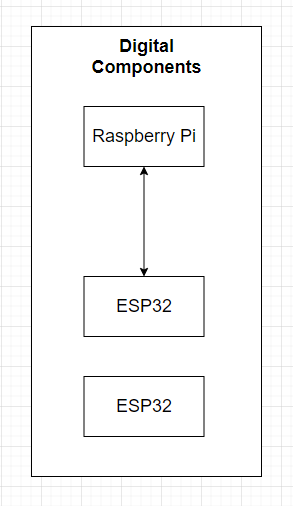
\includegraphics[scale=0.5]{images/digital_layer.PNG}
	\caption{Digital Components Layer}
\end{figure}
The Digital Components Layer is made up of the ESP32's and the Raspberry Pi. The ESP32 will receive data from the thermometer and will send the data to the Raspberry Pi. The Raspberry Pi will send the data to the web server and any instructions recieved from the web server will be sent to the ESP32's. The ESP32's will send a signal to the relay and activate the pumps and heating elements depending on which step of the brewing process it is in.

\subsection{Web Server Layer}

\begin{figure}[H]
	\centering
	\graphicspath{.\images}
	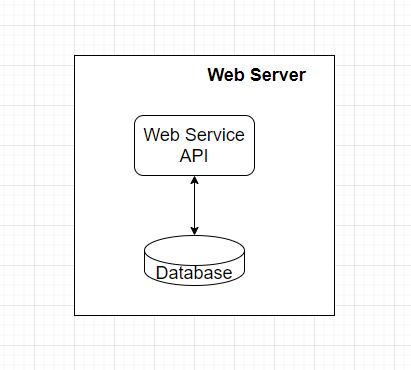
\includegraphics[scale=0.5]{images/web_layer.PNG}
	\caption{Web Server Layer}
\end{figure}
The Web Server Layer will be where all the data will be stored and instructions will be sent out from.  The web server will receieve data from the Raspberry Pi and will store the data in a database. The web server will then decide what actions the system must take in order to meet the criteria set by the brewer. The two primary actions that web server will control is activating the heating elements and the pumps. Conditions such as water temperature and the amount of time spent on a specific step of the brewing process will be receieved from the User Interface Layer and
will be maintained by the web server.

\subsection{User Interface Layer}

\begin{figure}[H]
	\centering
	\graphicspath{.\images}
	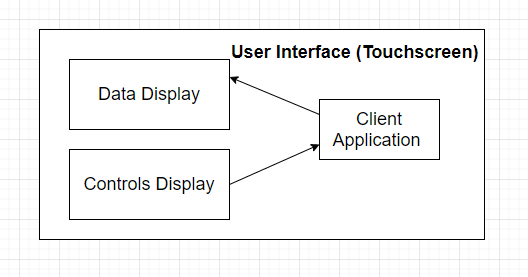
\includegraphics[scale=0.5]{images/ui_layer.PNG}
	\caption{User Interface Layer}
\end{figure}
The User Interface Layer will be where the user can set the conditions of the brewing system, as well as see the temperatures of the different kettles and the time remaining on the current step in the brewing process. The brewer will have a user interface which will allow them to set the temperatures of the HLT and the mash tun. The boiling kettle will not be set a specific temperature, instead the heating element will be set to a power output set by the brewer. Once the brewer has entered their desired conditions, this data will be sent to the web server through the client applciation.